\section{Method}
\label{sec:method}

\subsection{Overview}
Fig.~\ref{fig:architecture} shows the whole method. It runs in six stages and each stage answers one
question.

\begin{enumerate}
\item The frozen backbone produces a denoised image, and a small head estimates how confident the
backbone is at each pixel. This answers where the backbone is unsure.
\item Two small networks propose changes. One scales the image, the other adds detail back to
boundaries. This answers what change is available.
\item Six named clinical properties are measured on the backbone output. Each returns a score for the
image and a map of where it is unsatisfied. This answers what is wrong and where.
\item A rule layer turns those measurements into a per pixel allocation, which says how much of the
proposal to admit at each location. This answers where the change should be applied.
\item The admitted change is bounded, gated away from the background, smoothed and combined with the
edge term. This answers how the change is applied.
\item Three constraints are checked on the result, and the number that pass decides how much of the
candidate replaces the backbone output. This answers whether the change is allowed at all.
\end{enumerate}

The rest of this section takes the six stages in order.

\subsection{Stage one, the backbone and the confidence map}
\label{sec:confidence}
The backbone is frozen after training and gives $\mathbf{b} = f_\theta(\mathbf{y})$. A two layer
network $h_\phi$ reads a feature tensor $\mathbf{z}$ from inside it and produces the confidence map
\begin{equation}
\mathbf{c} = \sigma\!\left(\frac{h_\phi(\mathbf{z}) + \beta_0}{\tau_0}\right),
\label{eq:confidence}
\end{equation}
where $\sigma$ is the logistic function, $\tau_0 > 0$ is a learnable temperature and $\beta_0$ a
learnable offset. The uncertainty map is $\mathbf{u} = \mathbf{1} - \mathbf{c}$. A small temperature
gives a nearly binary map and a large one spreads the decision out.

Only this head depends on the backbone, because architectures expose feature tensors with different
channel counts. Table~\ref{tab:uncertainty_sources} lists the tensor used for each.
Everything after this stage is shared, which is the precise sense in which the method is modular
rather than architecture free. Section~\ref{sec:transfer_cost} reports what adapting this head costs.

\subsection{Stage two, the two correctors}
\label{sec:correctors}
Two changes are proposed, and they are deliberately of different kinds.

The \emph{gain} network proposes a multiplicative change. It runs at quarter resolution and emits a
brightness channel passed through a rectifier, so it can only brighten, and a contrast channel passed
through a hyperbolic tangent, so it can go either way. Their sum is scaled by $\alpha_{\max} = 0.15$
to give the raw gain $\boldsymbol{\Delta}$. A multiplicative form suits speckle, which is itself
multiplicative~\cite{goodman2007speckle}, so bright tissue receives a larger absolute change than dark
background for the same relative adjustment.

The \emph{edge} network proposes an additive change $\boldsymbol{\delta}_{\mathrm{e}}$ from four
channels, namely the intensity normalised residual, the edge magnitude of the backbone output, the
backbone output, and an unsharp mask. Its output is bounded to $\pm 0.08$ and scaled by a learned
factor. An additive form suits boundaries, which should be sharpened by the same amount in a bright
layer as in a dark one.

A third small network predicts a per pixel strength map $\boldsymbol{\lambda}$ with values in $[0,1]$
from the failure maps of Stage three. It modulates how much of the raw gain survives at each pixel.

\subsection{Stage three, the six clinical properties}
\label{sec:predicates}
The six properties are the interface between clinical language and the arithmetic of the method. Each
one is chosen because it names a way a denoised OCT image is known to fail, and each is written as a
formula so it can be recomputed by anyone.

Table~\ref{tab:predicates} gives, for every property, the clinical reason it exists, the score
$s_i \in [0,1]$ that summarises the whole image, the map $\mathbf{m}_i \in [0,1]^{H \times W}$ that
localises the failure, and the threshold $\tau_i$ that separates satisfied from unsatisfied. A larger
score means the property is better satisfied. A larger value of the map means stronger local evidence
that it is not.

None of these quantities needs a clean reference. They are computed from the noisy input and the
backbone output only, which is why they remain available at test time on a scanner the method has
never seen. Fig.~\ref{fig:predicate_maps} shows the six maps for one image.

\subsection{Stage four, the rule layer}
\label{sec:negotiator}
The rule layer decides where the gain proposal should act. It does so through five named rules, each
of which casts a signed vote.

Each property score is first turned into a soft failure signal by comparing it with its threshold,
\begin{equation}
f_i = \sigma\big(\kappa (\tau_i - s_i)\big), \qquad \kappa = 10 ,
\label{eq:soft_failure}
\end{equation}
so $f_i$ is near one when property $i$ is failing and near zero when it is satisfied. The constant
$\kappa$ sets how sharp that transition is. The same soft comparison is used to test the confidence
map and the strength of a proposal against their own thresholds. Conjunction uses the Lukasiewicz
form $\mathrm{AND}(a,b) = \max(0, a + b - 1)$, which is piecewise linear and has a bounded slope,
which is what makes the bound in Section~\ref{sec:stability} tight.

The five rules are the following. Rule one fires when the backbone is confident and the proposal is
weak, and it votes against changing the image. Rule two fires when the backbone is unsure and the
proposal is strong, and it votes for changing it. Rule three fires when a relevant property is
failing, and it votes for changing it. Rule four fires when confidence and proposal strength are both
middling, and it votes weakly for changing it. Rule five fires when several correctors want the same
pixel, and it votes against changing it. Write $r_1$ to $r_5$ for the resulting truth values.

The allocation at each pixel is the bounded weighted vote
\begin{equation}
\begin{aligned}
a ={}& \underbrace{B_{\min} + (B_{\max} - B_{\min})\,\sigma(\beta)}_{\text{base, no rule firing}} \\
    &- C_1 w_1 r_1 + C_2 w_2 r_2 + C_3 w_3 r_3 + C_4 w_4 r_4 - C_5 w_5 r_5 ,
\end{aligned}
\label{eq:allocation}
\end{equation}
where $\beta$ is a learnable base logit, $w_k = \sigma(\theta_k) \in (0,1)$ are learnable rule weights
and the budgets are $B_{\min} = 0.25$, $B_{\max} = 0.50$, $C_1 = 0.15$, $C_2 = 0.25$, $C_3 = 0.15$,
$C_4 = 0.10$ and $C_5 = 0.10$.

Those budgets are not arbitrary. They are chosen so that
$B_{\max} + C_2 + C_3 + C_4 = 1$ and $B_{\min} - C_1 - C_5 = 0$. Since every truth value lies in
$[0,1]$ and every weight lies in $(0,1)$, the value of Equation~\eqref{eq:allocation} already lies in
$[0,1]$ for every possible input and every possible parameter value. No clipping is ever needed. This
matters for two reasons. A clipped allocation would stop the gradient, so the rules could never be
trained, and a bound that is enforced by clipping would make the stability result in
Section~\ref{sec:stability} vacuous.

\subsection{Stage five, applying the change}
\label{sec:composition}
The admitted gain is the raw proposal modulated by the allocation and the strength map, then bounded,
\begin{equation}
\boldsymbol{\alpha} = \mathrm{clamp}\big(\boldsymbol{\Delta} \odot \mathbf{a} \odot \boldsymbol{\lambda},\, -0.20,\, 0.20\big).
\label{eq:alpha}
\end{equation}
A gate suppresses any change in the dark background,
\begin{equation}
\mathbf{g} = \sigma\big(20\,(\mathbf{b} - q_{0.15})\big),
\label{eq:gate}
\end{equation}
where $q_{0.15}$ is the fifteenth percentile of the backbone output of that image. Using a percentile
rather than a fixed level makes the gate work across scanners with different brightness.

The gated gain is applied multiplicatively, and the brightening part is smoothed before it is added
so that it cannot create a new high frequency edge,
\begin{equation}
\mathbf{v} = \big(\,\mathrm{smooth}(\mathrm{ReLU}(\boldsymbol{\alpha}) \odot \mathbf{b})
 + (\boldsymbol{\alpha} - \mathrm{ReLU}(\boldsymbol{\alpha})) \odot \mathbf{b}\,\big) \odot \mathbf{g},
\label{eq:apply}
\end{equation}
where $\mathrm{smooth}$ is a three by three mean filter. The darkening part is left unsmoothed because
it has zero mean and cancels itself. In the background, defined by the complement of the gate eroded
by two pixels, a masked three by three mean filter is blended in at half strength, which lowers the
background standard deviation without letting blur cross into tissue. Finally the edge proposal is
added and the result is clipped to the valid range,
\begin{equation}
\mathbf{q} = \mathrm{clamp}\big(\mathbf{b} + \mathbf{v} + \boldsymbol{\delta}_{\mathrm{e}} \odot \mathbf{g},\, 0,\, 1\big).
\label{eq:candidate}
\end{equation}

\subsection{Stage six, the safety decision}
\label{sec:safety}
The candidate $\mathbf{q}$ is not returned directly. Three constraints are checked on it.

\textbf{Aggregate quality must not fall.} Define the energy
\begin{equation}
E(\mathbf{v}) = 1 - \tfrac{1}{6}\sum_{i=1}^{6} s_i(\mathbf{v})
 + 0.1 \sum_{i=1}^{6} \max\big(0,\, 0.5 - s_i(\mathbf{v})\big),
\label{eq:energy}
\end{equation}
which is small when the image is good. The first constraint requires
$E(\mathbf{q}) \le E(\mathbf{b}) + 0.10$. The second term of Equation~\eqref{eq:energy} adds a penalty
for any single property that falls below one half, so a good average cannot hide one badly broken
property.

\textbf{No property may be sacrificed for another.} The second constraint requires that at least one
property improves by more than $0.01$ and that no property falls by more than $0.10$.

\textbf{The image must not move far.} The third constraint requires
$\lVert \mathbf{q} - \mathbf{b} \rVert_2 \,/\, \lVert \mathbf{b} \rVert_2 < 0.2$.

Let $n \in \{0,1,2,3\}$ be the number of constraints that hold. The output is
\begin{equation}
\hat{\mathbf{x}} = (1 - w)\,\mathbf{b} + w\,\mathbf{q},
\qquad
w = \begin{cases}
1, & n \ge 2, \\[2pt]
0.05 + 0.10\,\dfrac{n}{3}, & n < 2 .
\end{cases}
\label{eq:blend}
\end{equation}
When at least two constraints hold the candidate is accepted in full. When fewer hold the output
falls back almost entirely to the backbone, retaining between five and eight percent of the proposal
so that the decision remains visible in the output rather than silently discarded. This rule is
evaluated on every image at test time, and Section~\ref{sec:theory_check} reports how often each
constraint is the one that fails.


\begin{figure*}[!tb]
\centering
\includegraphics[width=\textwidth]{figures/architecture.pdf}
\caption{The six stages of the method. A frozen backbone produces the denoised image and a small head
estimates confidence. Two networks propose a multiplicative change and an additive edge change. Six
clinical properties are measured and produce a score and a failure map each. Five rules turn those
signals into a per pixel allocation. The admitted change is bounded, gated away from the background
and combined. Three constraints are then checked, and the number that pass decides how much of the
candidate replaces the backbone output.}
\label{fig:architecture}
\end{figure*}

\begin{table}[!tb]
\centering
\caption{Feature tensor read by the confidence head for each backbone. All heads share the same two
layer design and differ only in the number of input channels.}
\label{tab:uncertainty_sources}
\setlength{\tabcolsep}{4pt}
\footnotesize
\begin{tabular}{lll}
\toprule
Backbone & Feature tensor & Channels \\
\midrule
NAFNet & First encoder stage & 40 \\
KBNet & First encoder stage & 32 \\
DnCNN & First convolution & 228 \\
SwinIR & Shallow feature convolution & 138 \\
\bottomrule
\end{tabular}
\end{table}

\begin{table}[!tb]
\centering
\caption{The six clinical properties. Each one names a way a denoised OCT image is known to fail,
returns a score for the whole image and a map of where the property is unsatisfied, and is compared
against a threshold. The closed form of every score and every map is given in the supplementary file
and in the released code. Here $e$ is the Sobel edge magnitude of the backbone output, $\sigma_k$ is
the local standard deviation over a window of size $k$, and $cv$ is the local coefficient of
variation of the log residual.}
\label{tab:predicates}
\setlength{\tabcolsep}{3pt}
\footnotesize
\begin{tabular}{clp{0.40\columnwidth}c}
\toprule
$P_i$ & Property & Where the map is large & $\tau_i$ \\
\midrule
$P_1$ & edge continuity & away from detected edges, where a boundary should continue but does not & 0.60 \\
$P_2$ & local contrast & where $\sigma_9$ falls below the image mean, and in nearly flat tissue & 0.50 \\
$P_3$ & flat smoothness & inside flat regions that still carry residual variation & 0.75 \\
$P_4$ & structural coherence & where the edge map is itself rough, a sign of broken structure & 0.50 \\
$P_5$ & speckle conformity & where $cv$ departs from the value expected for OCT speckle & 0.30 \\
$P_6$ & layer visibility & where the local variance of the edge map is high across depth & 0.70 \\
\bottomrule
\end{tabular}
\end{table}

\begin{figure*}[!tb]
\centering
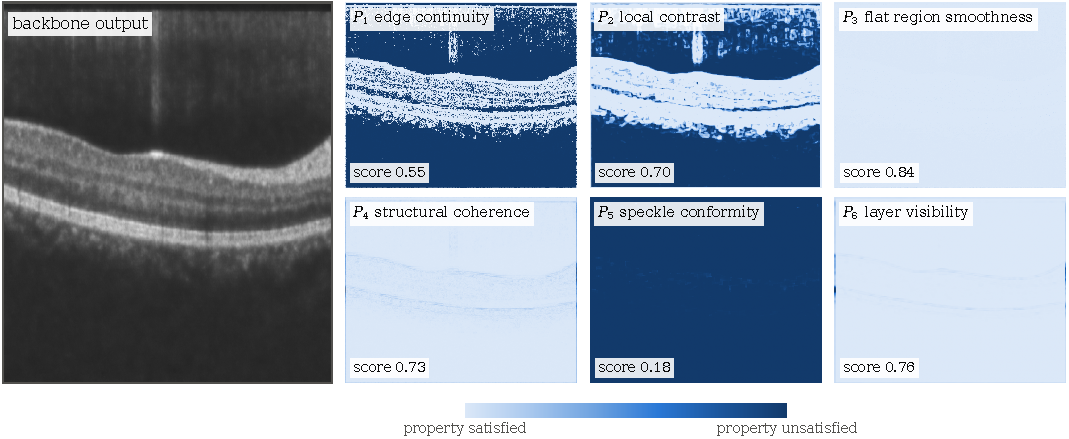
\includegraphics[width=0.98\textwidth]{figures/fig_predicate_maps.pdf}
\caption{The six clinical properties on one backbone output. Each panel shows where that property is
locally unsatisfied, on a shared scale, with the image level score in the corner. Edge continuity,
local contrast and speckle conformity carry most of the evidence on this image, while the other three
are close to satisfied everywhere.}
\label{fig:predicate_maps}
\end{figure*}
